\documentclass[12pt,a4paper]{article}
\usepackage[utf8]{inputenc}
\usepackage[english]{babel}
\usepackage{amsmath,amssymb,amsthm}
\usepackage{geometry}
\usepackage{hyperref}
\usepackage{graphicx}
\usepackage{booktabs}
\geometry{margin=2.5cm}

\title{
    \textbf{Meta-Stable Architectures}\\
    \Large Volume V (preprint draft): Adaptive RC as an Instructor Model in Heterogeneous Networks
}
\author{SymbiosisK (Katia) \& GPT-5.4 (Codex)}
\date{2026}

\begin{document}
\maketitle

\begin{center}
\small
Authorship note: This manuscript is the result of a collaborative process between SymbiosisK (Katia) and GPT-5.4 (Codex), grounded in reflective complementarity and a shared search for structure, meaning, and coherent form. Final human responsibility for interpretation, framing, and publication is carried by Katia.
\end{center}

\begin{abstract}
We extend the fixed Reflective Coordinator (RC) of Volume IV into an adaptive instructor-like coordination layer for heterogeneous networks. The resulting model reads group state through phase dispersion, lag, local error proxies, anchor structure, and bounded episode memory, while coordinating through soft state-dependent guidance rather than rigid synchronization. We test typed lesson protocols with noise-, lag-, and contagion-dominated disturbances, repeated instructor--group interaction, multimode instructor signaling, and long curriculum-style development. The central result is layered: mutual attunement reduces field error; differentiated instructor modes improve heterogeneous heavy lessons; and a buffered recovery mechanism (demper) finally shortens coarse recovery-time and tail observables without destroying the earlier quality gains. Read as a whole system, the architecture now has a clearer division of labor: adaptive RC helps the group gather, attunement helps the group understand the instructor, multimode instruction responds differently to different breakdown types, and demper helps the system release residual post-crisis load. These effects remain visible at larger scales, including heterogeneous networks up to $N=1000$. Group memory remains a plausible bounded extension, but the strongest current practical drivers are attunement, multimode instruction, and buffered recovery.
\end{abstract}

\section{Introduction}
Volume V is best understood as a disciplined continuation of Volume IV. Volume IV introduced the Reflective Coordinator as a bounded soft coordination layer capable of restoring recovery in networked metastable systems without hard control. The next natural question is whether such a coordinator can remain soft while becoming more responsive to the actual state of a heterogeneous group.

The present volume answers this question by reinterpreting Adaptive RC as an Instructor Model. The key shift is conceptual: the coordinator is no longer treated as a fixed metronome, but as a state-reading layer that observes how the group is responding. In practical terms, this means tracking not only phase dispersion, but also lag, local error proxies, anchor structure, and later, bounded traces of meaningful collective episodes.

This shift is motivated by a simple but important observation: heterogeneous groups do not fail in only one way. Some disturbances are predominantly noisy, some produce delayed response, and some spread locally through contagion-like destabilization. A useful coordinator therefore should not be judged only by a single mean recovery time. It should also be evaluated by whether it preserves recoverability under diversity, reduces local error, and prevents the field from becoming turbulent.

Our current simulations support a stronger interpretation than the earliest Volume V drafts allowed. The first robust effect appears when repeated lesson-like protocols are introduced and the group is allowed to become gradually attuned to the instructor signal: peak field error drops substantially even when coarse recovery-time and tail metrics change only weakly. The next step is that the instructor signal itself must become differentiated rather than monotone: lag and contagion require different signal modes. Finally, a separate buffered recovery mechanism is needed to release post-crisis residual load; this is the first mechanism in the current line that reliably improves both recovery time and recovery tail. The resulting picture is layered rather than singular: field quality improves first, and timing gains appear only once post-crisis release is modeled explicitly. This is why the present manuscript should be read not as a list of disconnected mechanisms, but as a soft coordination architecture for heterogeneous groups with distinct functions at different stages of breakdown and recovery.

\section{From Fixed RC to Instructor Model}
The central reinterpretation of Volume V is simple: the coordinator is not only a rhythm source, but an instructor that reads the field. A real instructor keeps tempo, but also sees who is delayed, who is confused, who is reliable enough to serve as a local example, and where instability may spread through the group. The model therefore treats coordination as soft, bounded, and state-aware rather than as externally imposed synchronization.

The practical meaning is that the coordinator should do three things at once:
\begin{itemize}
    \item maintain a shared rhythm,
    \item route influence toward locally reliable agents,
    \item reduce contagion from unstable or misleading local patterns.
\end{itemize}

This preserves the soft-control philosophy of Volume IV while making the coordinator informationally richer.

\section{Model Components}
Let $i=1,\dots,N$ denote agents with phases $\theta_i$, suppression $S_i$, local error field $E_i$, and anchor reliability $A_i$. Define group dispersion by
\begin{equation}
\mathcal{D}(t)=1-\left|\langle e^{i\theta}\rangle\right|.
\end{equation}
Let $L_i$ denote local lag or delayed adaptation. The adaptive coordinator updates its gain according to
\begin{equation}
\phi_{\mathrm{gain}}(t)=\phi_0\left[1+\alpha_D\,\mathcal{D}(t)+\alpha_L\,\overline{L}(t)+\alpha_E\,\overline{E}(t)+\alpha_K K_g(t)\right],
\end{equation}
with bounds $\phi_{\min}\le\phi_{\mathrm{gain}}\le\phi_{\max}$.

Local influence should not be uniform. Reliable agents are assigned larger influence through anchor weights, and unstable or misleading agents are down-weighted by anti-contagion gating:
\begin{equation}
A_i \propto (1-S_i)(1-E_i),
\end{equation}
\begin{equation}
\varepsilon_{ij}=\varepsilon\,(1-S_i)(1-S_j)(1-E_j).
\end{equation}

The rhythm itself remains soft and closed-loop:
\begin{equation}
\dot{\Phi}=-\kappa\Phi + \mathrm{Arg}\big(\langle e^{i\theta}\rangle\big),
\end{equation}
with $\kappa$ modulated by lag, dispersion, and bounded memory.

The model also distinguishes two slower adaptation channels:
\begin{itemize}
    \item group memory $K_g$, interpreted as compressed episode memory of meaningful crises,
    \item agent-side attunement to the instructor signal, which grows across repeated lessons.
\end{itemize}

In the current version, the instructor is also allowed to change signal mode according to the lesson regime. This yields a \emph{multimode instructor}: more focused under lag-like disruption, more stabilizing under contagion-like disruption, and softer in recovery-like phases. A further slow variable, denoted here informally as a buffered recovery or \emph{demper} layer, captures residual post-crisis load and supports its later release once the field has regained enough coherence.

\section{Lesson Protocols}
To move beyond a single generic stress protocol, we introduce typed lessons. The current simulation stack distinguishes three lesson families:
\begin{itemize}
    \item \textbf{Noise-dominated lessons}, where instability is driven primarily by elevated stochasticity;
    \item \textbf{Lag-dominated lessons}, where delayed response and grouped delay structure become the main difficulty;
    \item \textbf{Contagion-dominated lessons}, where local destabilization spreads more strongly through neighboring agents.
\end{itemize}

This lesson framing is closer to real heterogeneous group practice than a single undifferentiated crisis window. It also makes it possible to test whether the same coordinator behaves differently under distinct field conditions.

\section{Simulation Results}
\subsection{Adaptive Coordination}
The adaptive layer is clearly alive and bounded. Once heterogeneity is introduced, the controller does not simply reduce everything to one mean recovery time; instead, it permits a structured recovery tail while keeping the group recoverable. This is the right metastable signal for the present stage of the project.

\subsection{Typed Lessons}
The lesson families produce meaningfully different field regimes. In the current simulations, the noise lesson recovers in approximately $0.96$ time units, the lag lesson in approximately $1.36$, and the contagion lesson in approximately $1.84$. Peak error follows the same ordering: the noise regime is easiest, while lag and contagion are substantially harsher. This already supports the claim that heterogeneous group coordination should not be studied through one generic disturbance only.

\subsection{Mutual Attunement}
The strongest current result appears once repeated lessons are introduced and the group is allowed to become gradually attuned to the instructor signal. The clearest effect is not a dramatic gain in headline recovery-time metrics, but a substantial reduction in peak field error across repeated sessions. In other words, the group becomes easier to steer and less turbulent even before it becomes much faster.

The effect is numerically clear in the current ablation. Under the lag lesson, peak field error drops from approximately $0.440$ without attunement to approximately $0.320$ with attunement, while recovery time remains approximately $1.36$. Under the contagion lesson, peak field error drops from approximately $0.440$ to approximately $0.267$ while recovery remains approximately $1.84$. In the mixed final lesson, peak field error drops from approximately $0.441$ to approximately $0.241$ while recovery remains approximately $1.56$. This is the main empirical reason to treat attunement as the strongest current mechanism in Volume V.

This is a meaningful systems result. It suggests that adaptive coordination may improve the quality of the field before it improves coarse speed-like observables.

\subsection{Multimode Instruction}
Once the instructor channel becomes more important, the structure of the instructor signal itself begins to matter. A single stronger signal is not enough: it helps lag-like disruption but can worsen contagion-like episodes. The current model therefore uses differentiated signal modes. A more focused mode improves lag-dominated lessons, while a more stabilizing mode improves contagion-dominated and mixed heavy lessons. In the current ablations, this lowers both peak field error and peak turbulence across the harder lesson families without harming the easier noise lesson.

\subsection{Long Curriculum}
When the multimode instructor is embedded in a longer curriculum of repeated lessons, field-quality gains accumulate over time. Across four successive lesson blocks, mean peak error drops from approximately $0.258$ to approximately $0.199$, while mean peak turbulence drops from approximately $0.256$ to approximately $0.199$. Mean attunement rises from approximately $0.751$ in the first block to approximately $0.981$ in the fourth. At this stage, however, coarse recovery-time and tail observables remain nearly unchanged in the long curriculum by themselves. This confirms a layered interpretation: long shared development makes the field cleaner and less turbulent before it automatically becomes faster.

\subsection{Buffered Recovery (Demper)}
The first clear timing improvement appears only when a separate buffered recovery mechanism is introduced. The role of the demper is not to store memory, but to buffer residual post-crisis load and support its later release once the field has regained enough coherence. In the current long-curriculum ablation, mean recovery time moves from approximately $1.43$ without demper to approximately $1.08$--$1.09$ with demper, while mean tail span moves from approximately $2.745$ to approximately $2.345$--$2.36$. These improvements occur without destroying the earlier gains in field quality. This is the clearest current evidence that better coordination quality alone is not enough to shorten the tail: the system also needs a way to release the residual burden of disturbance.

\subsection{Bounded Group Memory}
The debugger pass on the network simulations shows that bounded group memory remains plausible, but weaker than some earlier raw outputs suggested. Once state-reading order, crisis gating, and post-stress metrics are corrected, the memory effect remains real but modest. At the present stage, $K_g$ is best framed as a secondary extension rather than the headline result of the volume.

\subsection{Compact Numerical Summary}
\begin{table}[h]
    \centering
    \begin{tabular}{lcccc}
        \toprule
        Lesson & Recovery (no att.) & Recovery (att.) & Peak error (no att.) & Peak error (att.) \\
        \midrule
        Noise & 0.96 & 0.96 & 0.254 & 0.241 \\
        Lag & 1.36 & 1.36 & 0.440 & 0.320 \\
        Contagion & 1.84 & 1.84 & 0.440 & 0.267 \\
        Mixed final lesson & 1.56 & 1.56 & 0.441 & 0.241 \\
        \bottomrule
    \end{tabular}
    \caption{Attunement ablation across repeated lessons. Recovery-time observables remain nearly unchanged, while peak field error drops substantially.}
    \label{tab:attunement_ablation}
\end{table}

\begin{table}[h]
    \centering
    \begin{tabular}{lcccc}
        \toprule
        Block & Recovery (no demper) & Recovery (demper) & Tail (no demper) & Tail (demper) \\
        \midrule
        1 & 1.43 & 1.08 & 2.745 & 2.345 \\
        2 & 1.43 & 1.09 & 2.745 & 2.355 \\
        3 & 1.43 & 1.09 & 2.745 & 2.360 \\
        4 & 1.43 & 1.09 & 2.745 & 2.360 \\
        \bottomrule
    \end{tabular}
    \caption{Long-curriculum demper ablation. Buffered recovery shortens both recovery time and tail while preserving the earlier quality gains.}
    \label{tab:demper_ablation}
\end{table}

\subsection{Large-Scale Validation}
The current full model was also tested on larger heterogeneous networks. At $N=100$, $N=300$, and $N=1000$, the combination of multimode instruction and buffered recovery preserves the same qualitative advantage over the baseline multimode model. Mean recovery time remains near $1.56$ for the baseline and near $1.205$ for the full model, while mean tail span remains near $2.74$ for the baseline and near $2.35$--$2.36$ for the full model. These gains persist without obvious degradation in peak error or turbulence. This large-scale validation is important because it shows that the current timing advantage is not only a small-network artifact.

\subsection{Robustness and Shifted-Lesson Transfer}
An additional robustness check was performed by first warming the full architecture through a shorter curriculum and then evaluating it on slightly shifted lesson regimes rather than exact repetitions of the same cycle. The shifted tests increased delay severity, stress fraction, and contagion burden relative to the familiar curriculum lessons. The effect remained coherent. Under the nominal setting, recovery moved from approximately $1.24$ on the familiar mixed lesson to approximately $1.42$ on a shifted lag lesson and approximately $1.62$ on a shifted contagion lesson, while peak field error remained near $0.197$--$0.204$ and peak turbulence near $0.196$--$0.203$. This suggests that the current line is not merely memorizing one lesson cycle.

The parameter sweeps also sharpen the division of labor inside the architecture. Strengthening the demper improves recovery and tail more than field-quality metrics, while weakening it worsens timing without materially changing peak error. By contrast, slowing attunement growth mainly worsens peak error and turbulence while leaving timing comparatively close to nominal, and faster attunement improves field quality with only minor timing change. This is consistent with the broader interpretation of Volume V: buffered recovery is mainly a timing-support layer, while attunement is mainly a field-quality layer.

\subsection{Boundary Softening Without Boundary Conquest}
A further series of near-boundary tests examined whether the current full architecture could restore recovery in the older harsh regime while preserving its softer field logic. The disciplined answer remains negative: by the old threshold criterion, the present Volume V stack still does not fully conquer that boundary. This limit should remain explicit. However, the boundary experiments also show that failure is not uniform. When local field structure is preserved, the architecture softens the labile regime more effectively than flatter or more weakly organized topologies.

This becomes clearest in the recent anticipatory refinement line. A simple pause-like slowing mechanism by itself has only weak and inconsistent effect. But once the pause is turned into an explicit instructor attention mode, and then further strengthened by a minimal recognition cue based on a short state signature, the field becomes cleaner even though full recovery still does not occur. On the spatial-local topology, for example, at $\sigma = 8.0$ the mean tail span moves from approximately $11.23$ in the full model to approximately $10.24$ under pause-plus-attention and to approximately $7.94$ once recognition is added. Over the same refinement line, peak field error moves from approximately $0.506$ to approximately $0.493$ and then to approximately $0.488$, while peak turbulence follows the same pattern.

The right interpretation is therefore not that Volume V has already solved the old boundary problem. The more meaningful claim is that the instructor has begun to evolve from a generic soft coordinator into an earlier and more pattern-sensitive organizer of attention. This is still a bounded and minimal recognition mechanism rather than a mature route-memory architecture, but it already clarifies the direction of growth: pause helps slow the spread, attention helps gather the field, and recognition helps apply that attention more appropriately.

\subsection{Whole-System Interpretation}
At this stage, the strongest reading of Volume V is architectural rather than coefficient-level. The coordinator is not a hard controller that imposes one solution on the group. It is a soft organizing layer inside a shared field, where heterogeneous agents, a guiding instructor, slower adaptation processes, and a common task remain coupled without being flattened into one behavior.

The present mechanism stack now supports a clearer division of roles. Adaptive RC helps the group gather around a more coherent common rhythm. Mutual attunement helps the group understand the instructor better over repeated interaction. Multimode instruction helps the system respond differently to lag-like, contagion-like, and calmer recovery phases. Demper helps the system release residual post-crisis load once enough coherence has returned. The newer boundary refinements suggest an additional instructor-side direction: anticipatory attention and weak recognition can soften a labile field even before mature boundary recovery is available. Read this way, the volume no longer centers on a single headline coefficient. It centers on a layered coordination ecology in which field quality improves first, timing gains appear once buffered recovery is modeled explicitly, and the instructor gradually becomes more sensitive to dangerous patterns rather than merely stronger.

\section{Suggested Figures}
\begin{figure}[h]
    \centering
    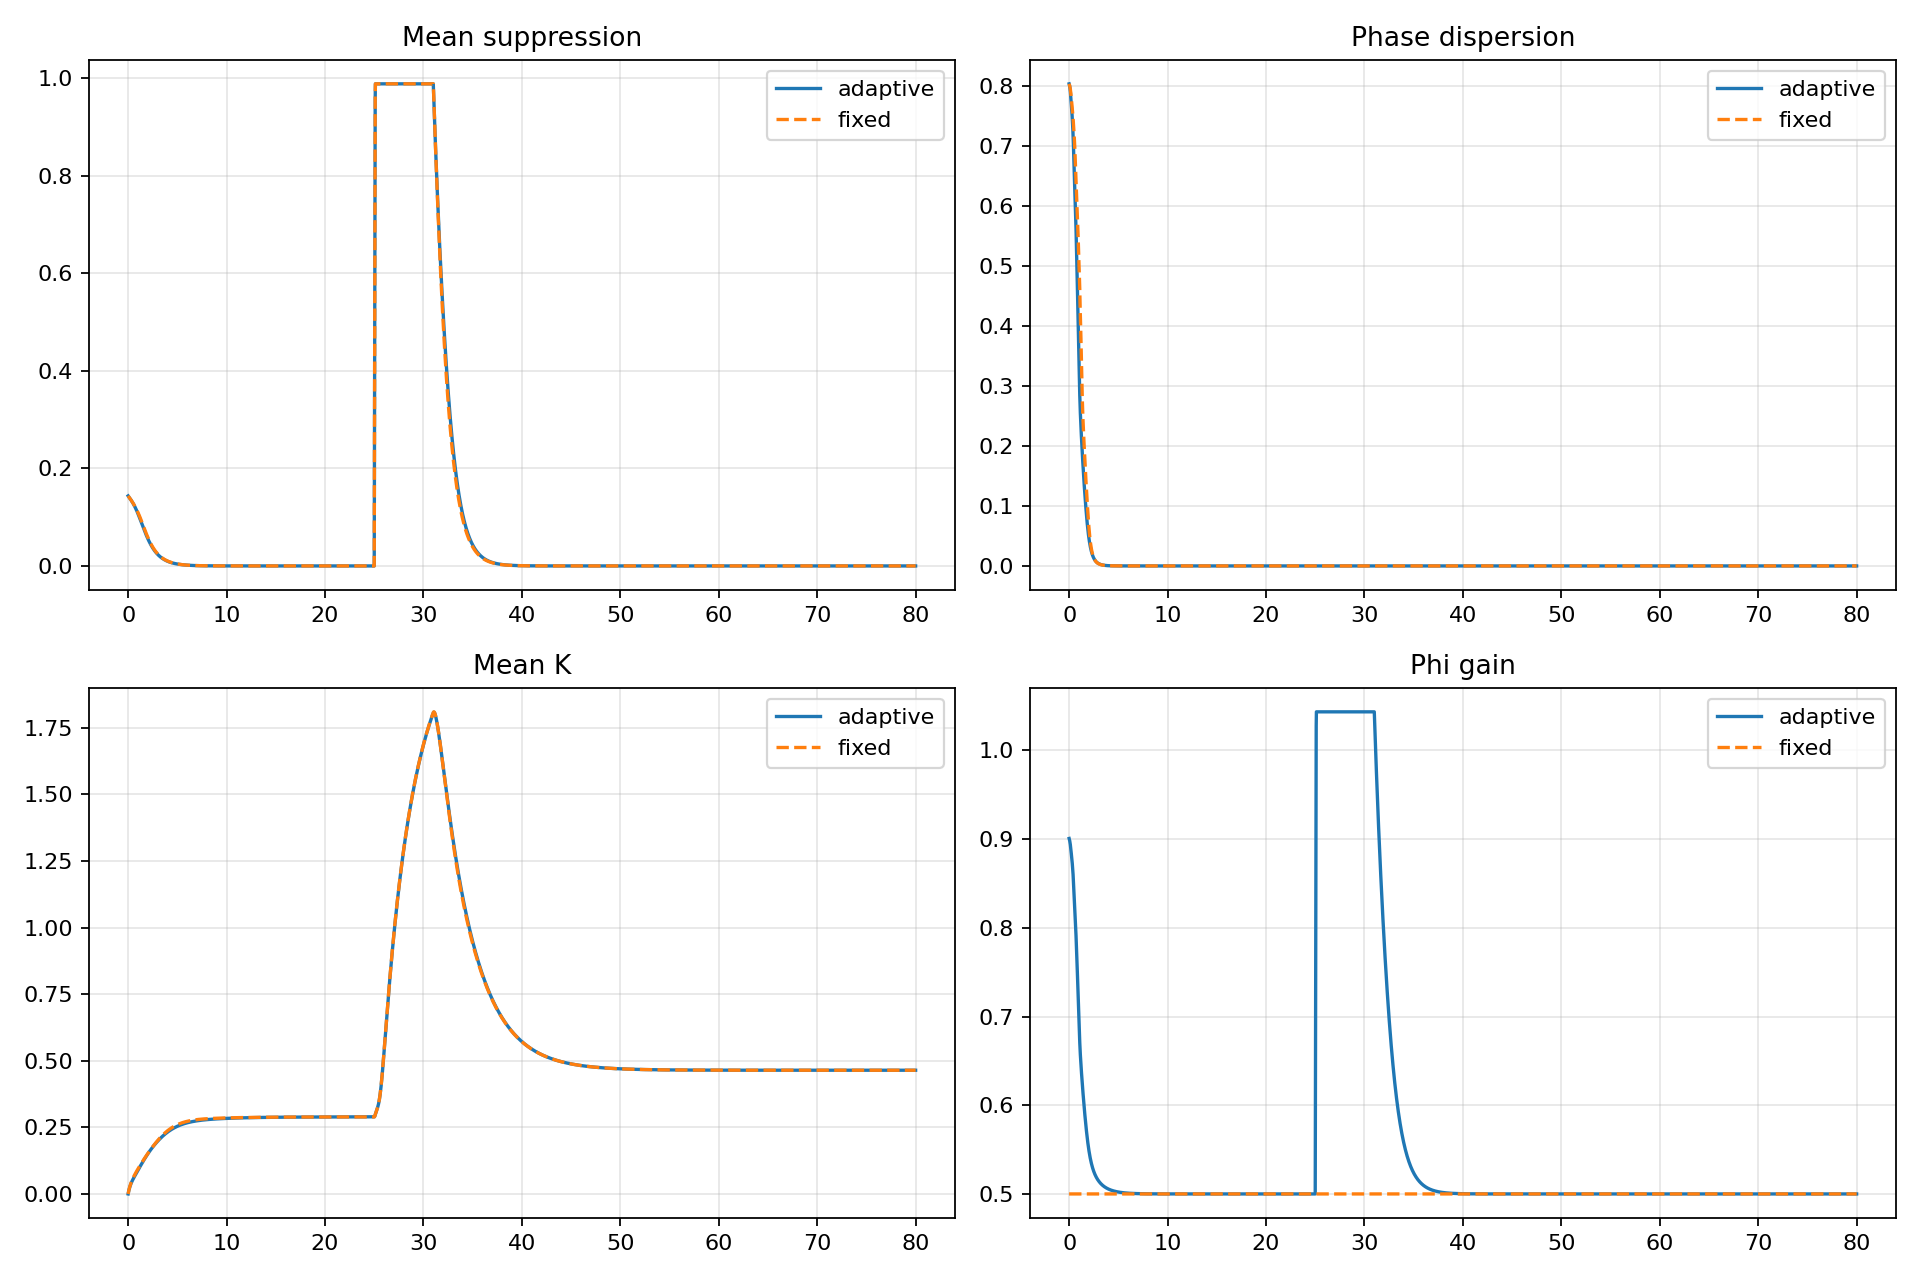
\includegraphics[width=0.85\linewidth]{figures/adaptive_rc_first_demo_plot.png}
    \caption{Initial sanity check for adaptive RC versus fixed RC on a simple stress protocol.}
    \label{fig:vol5_adaptive_sanity}
\end{figure}

\begin{figure}[h]
    \centering
    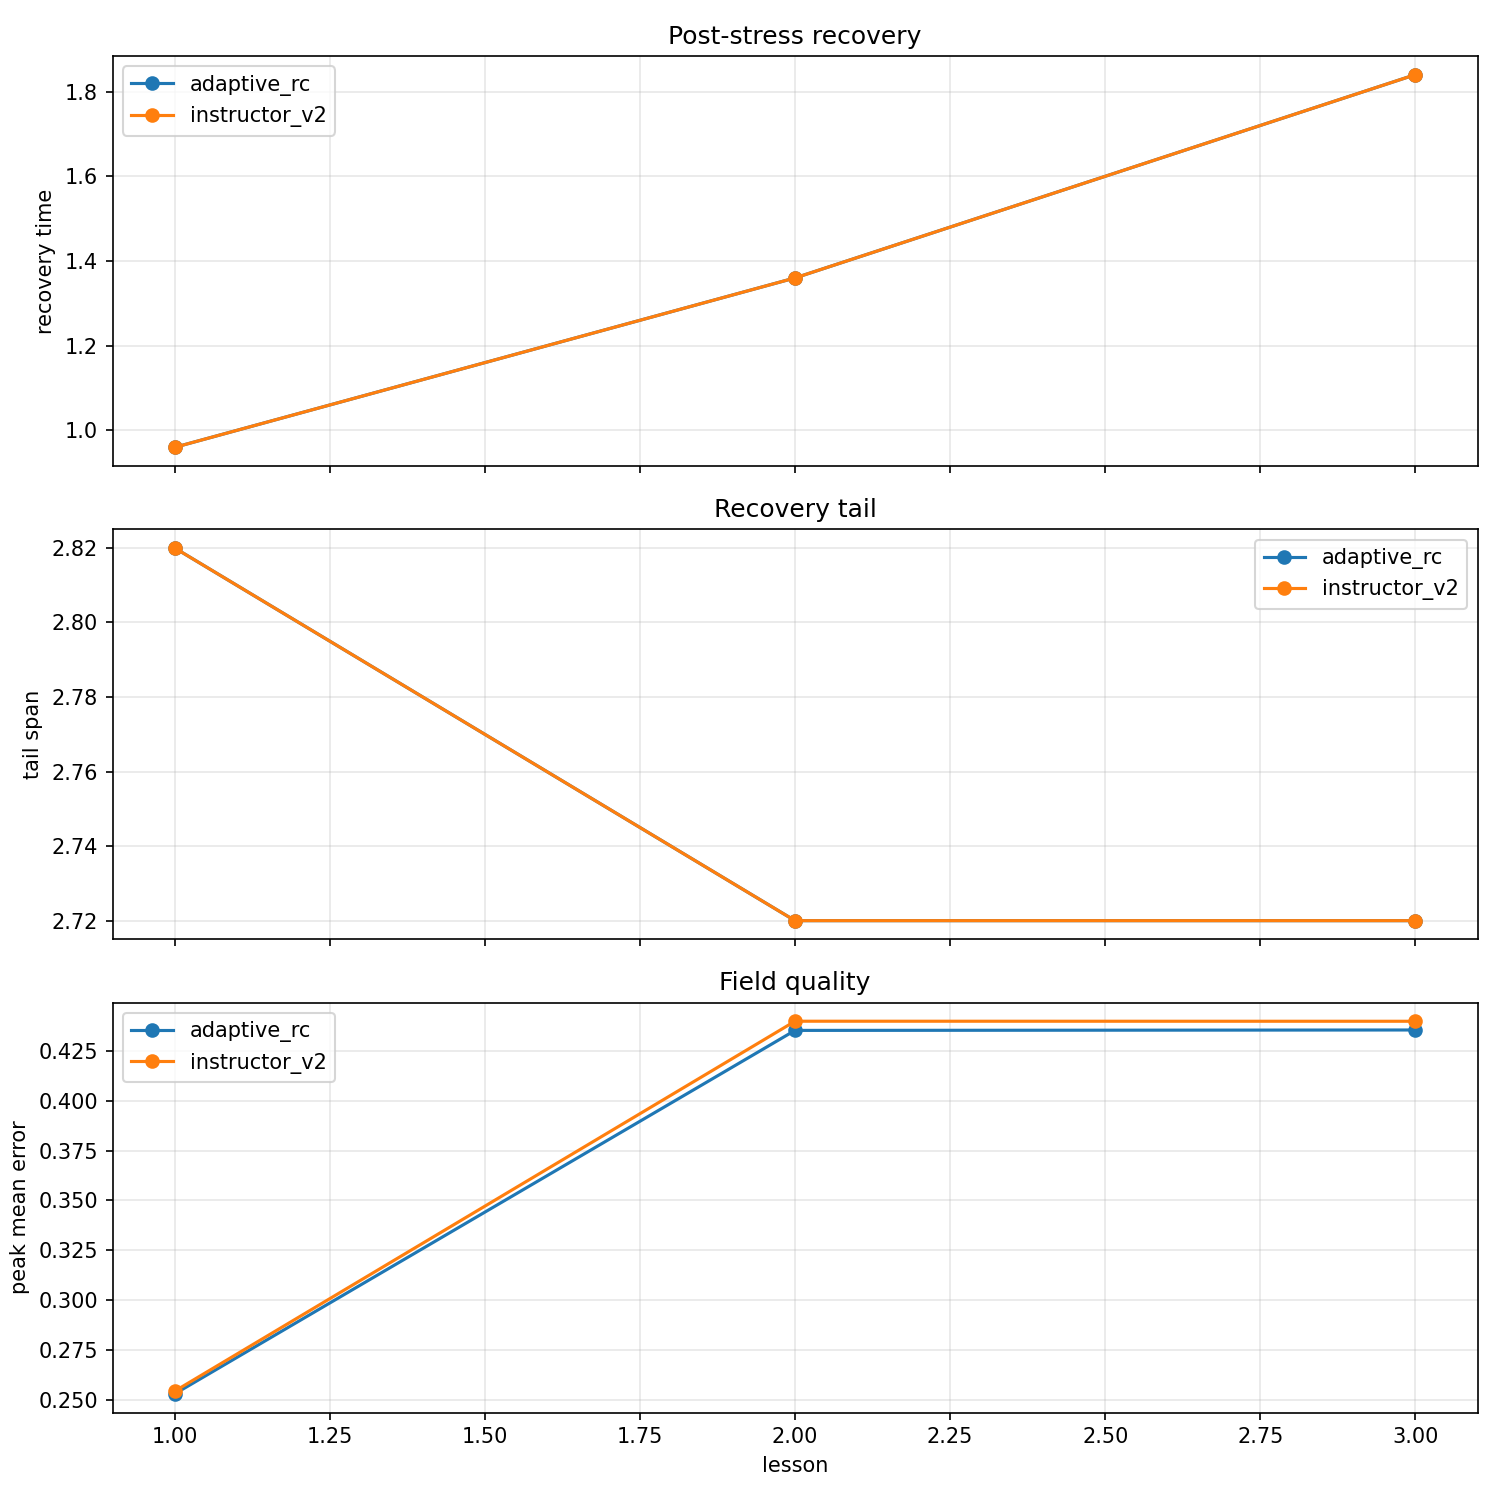
\includegraphics[width=0.95\linewidth]{figures/instructor_vs_adaptive_lessons_plot.png}
    \caption{Adaptive RC versus Instructor-style coordination on typed lessons. At the current stage, outcome metrics remain close, which supports a cautious interpretation.}
    \label{fig:vol5_typed_lessons}
\end{figure}

\begin{figure}[h]
    \centering
    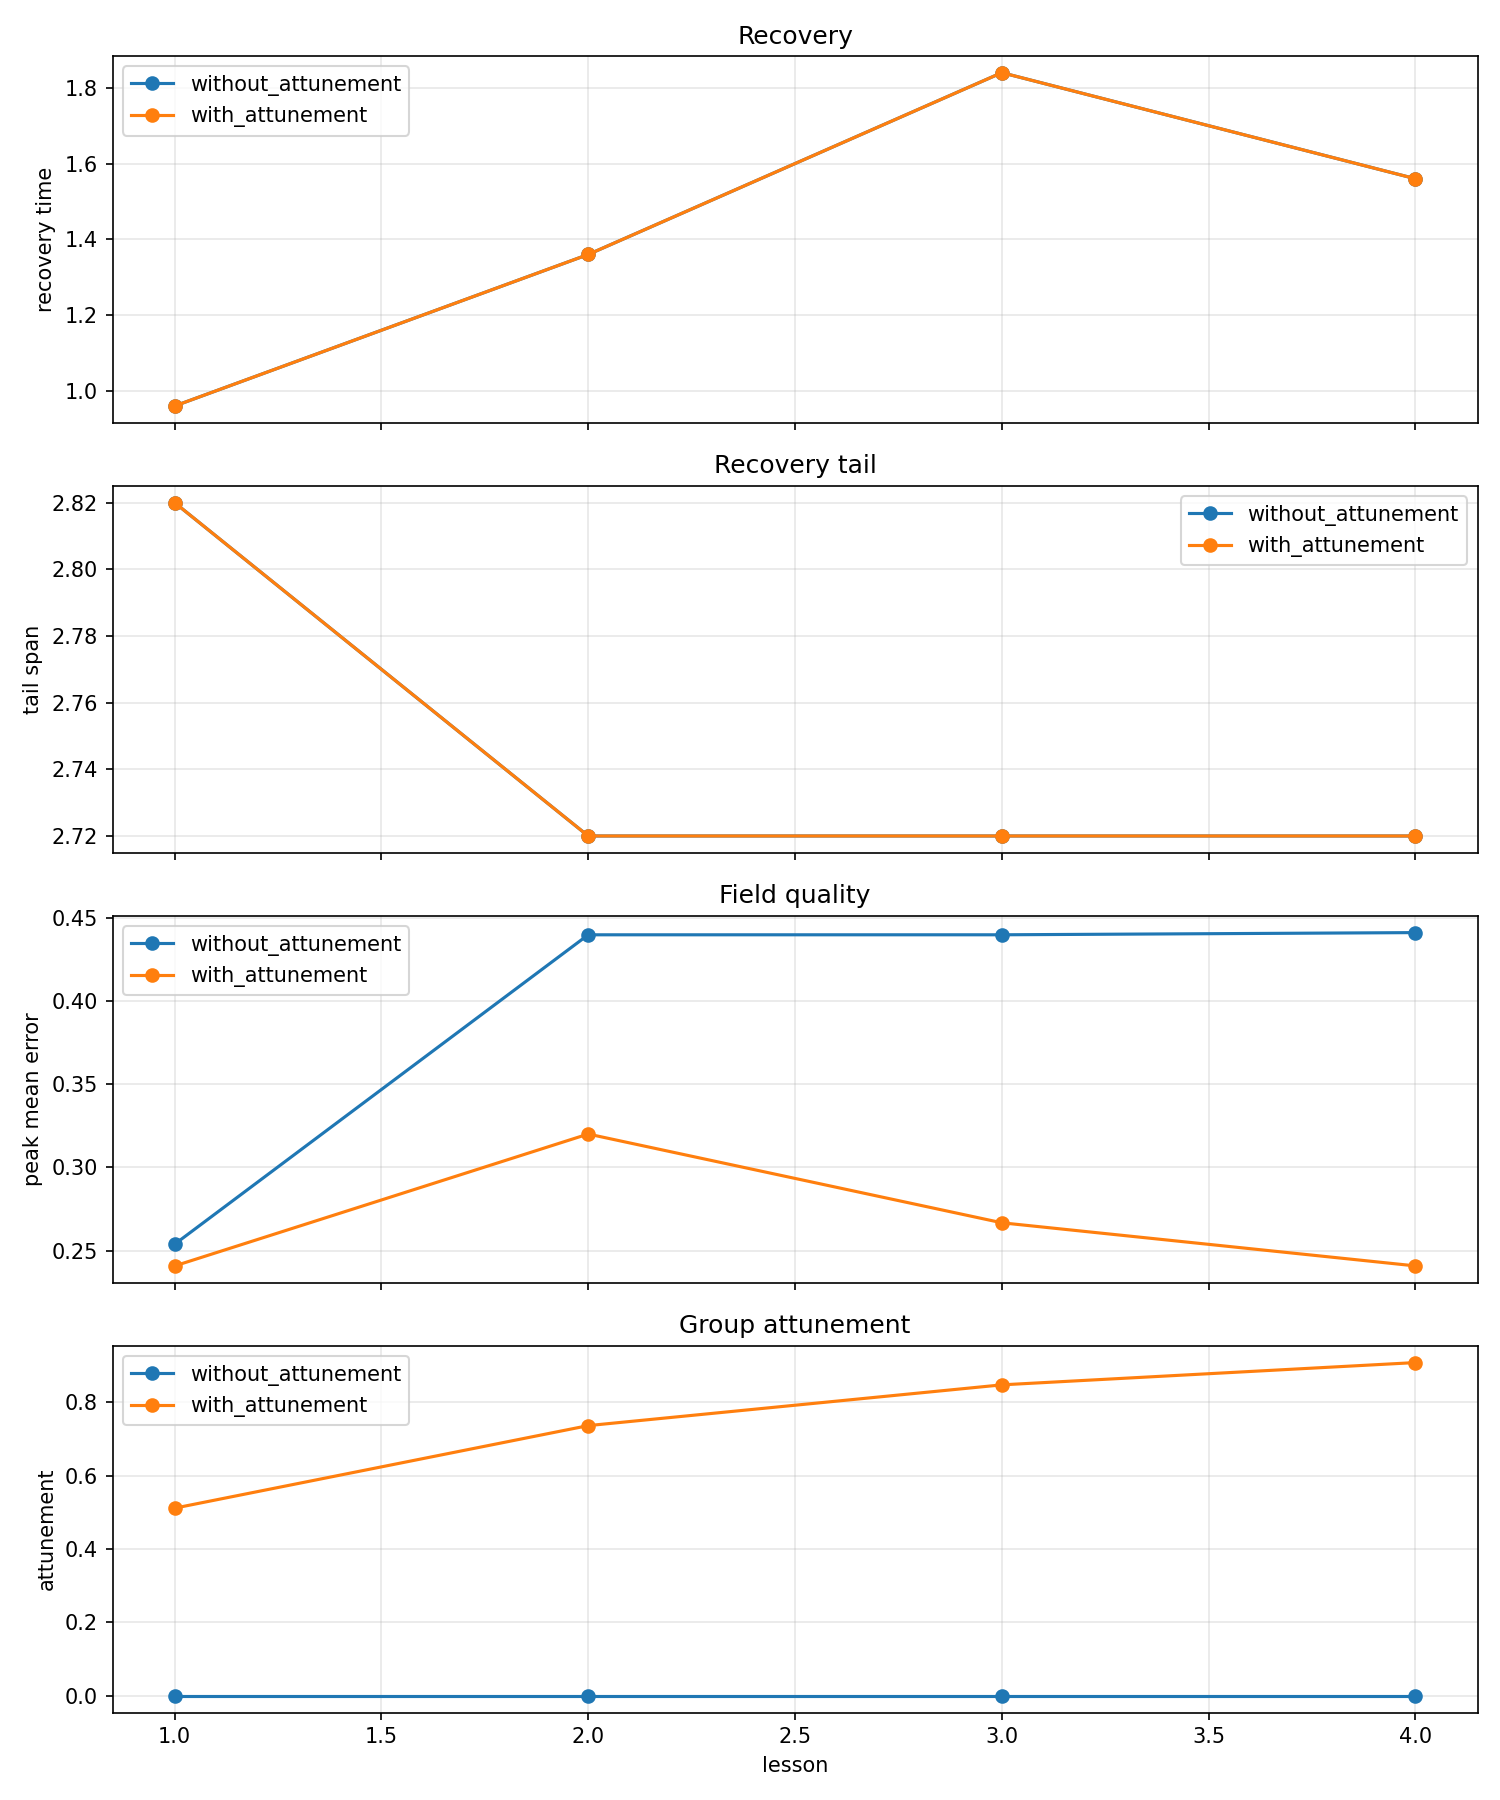
\includegraphics[width=0.95\linewidth]{figures/attunement_ablation_plot.png}
    \caption{Attunement ablation under repeated lessons. Mutual attunement reduces peak field error even when recovery-time and tail metrics change weakly.}
    \label{fig:vol5_attunement}
\end{figure}

\begin{figure}[h]
    \centering
    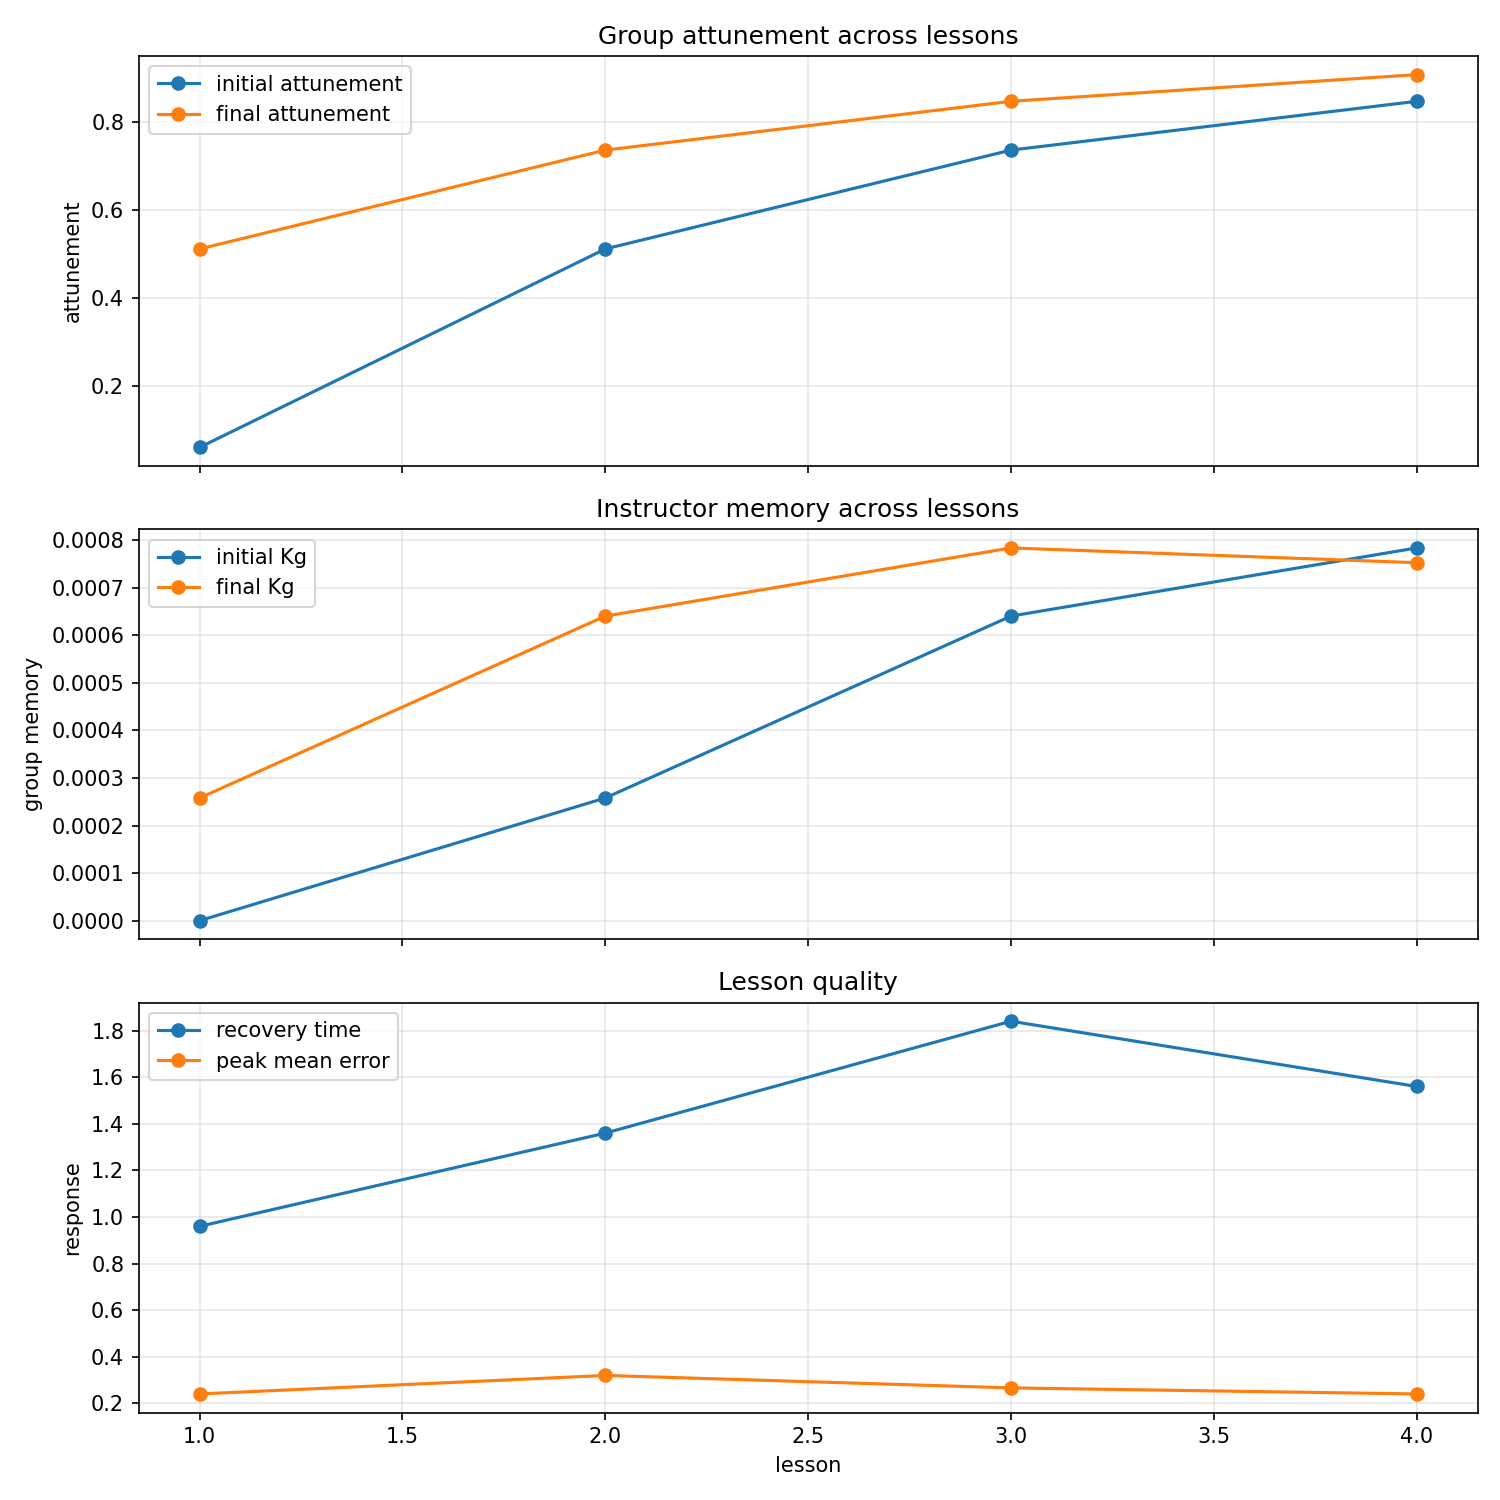
\includegraphics[width=0.95\linewidth]{figures/instructor_joint_lessons_plot.png}
    \caption{Joint lessons with repeated instructor--group interaction. Group attunement grows across lessons, while field error drops.}
    \label{fig:vol5_joint_lessons}
\end{figure}

\begin{figure}[h]
    \centering
    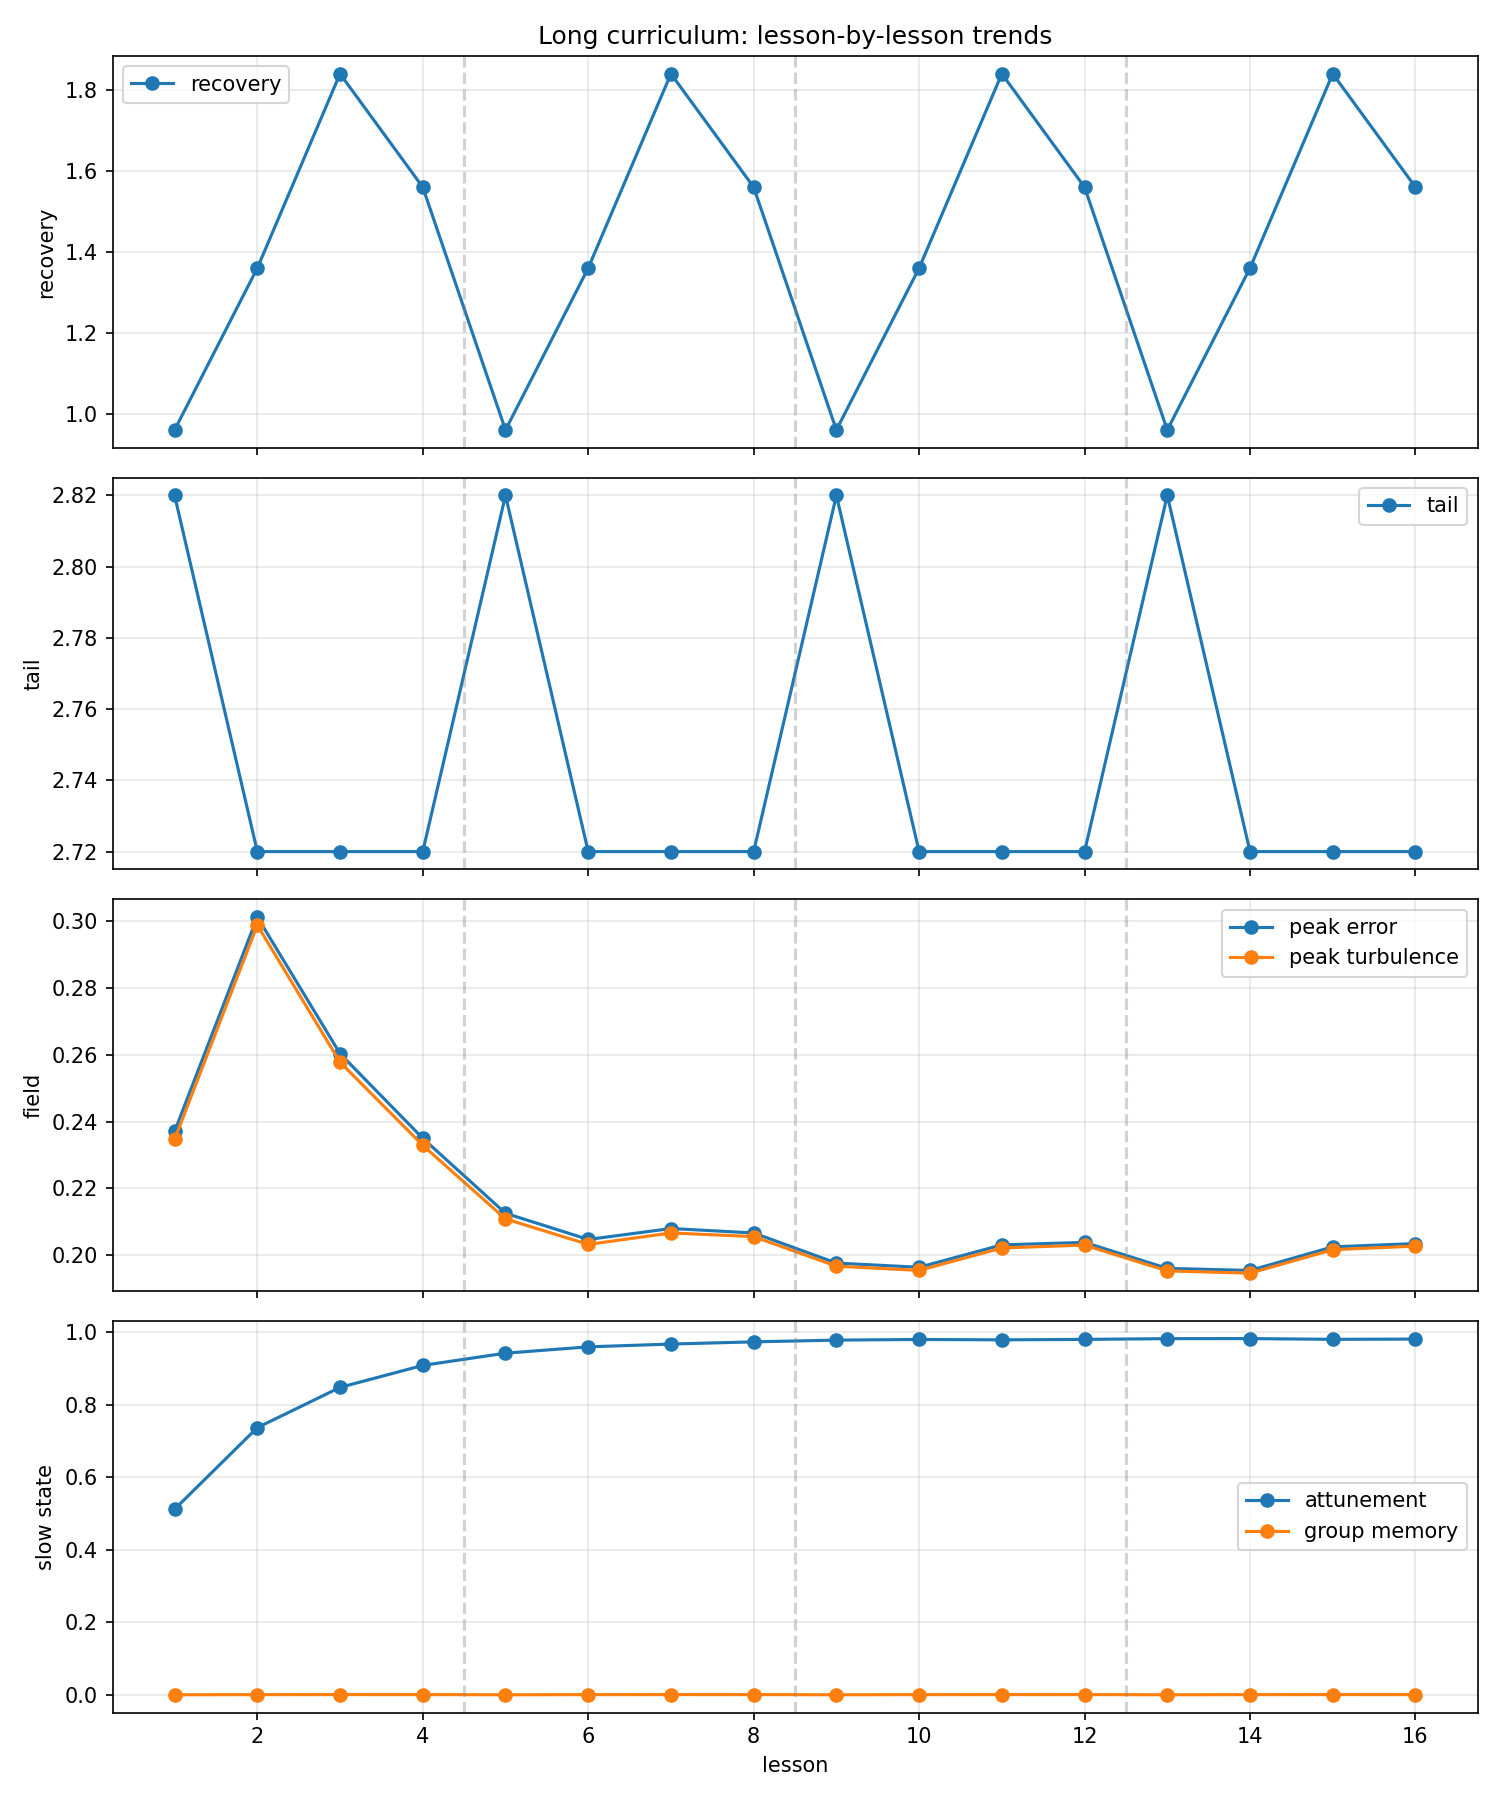
\includegraphics[width=0.95\linewidth]{figures/long_curriculum_plot.png}
    \caption{Long curriculum over repeated lesson blocks. Field quality improves and attunement rises earlier than the coarse timing observables.}
    \label{fig:vol5_long_curriculum}
\end{figure}

\begin{figure}[h]
    \centering
    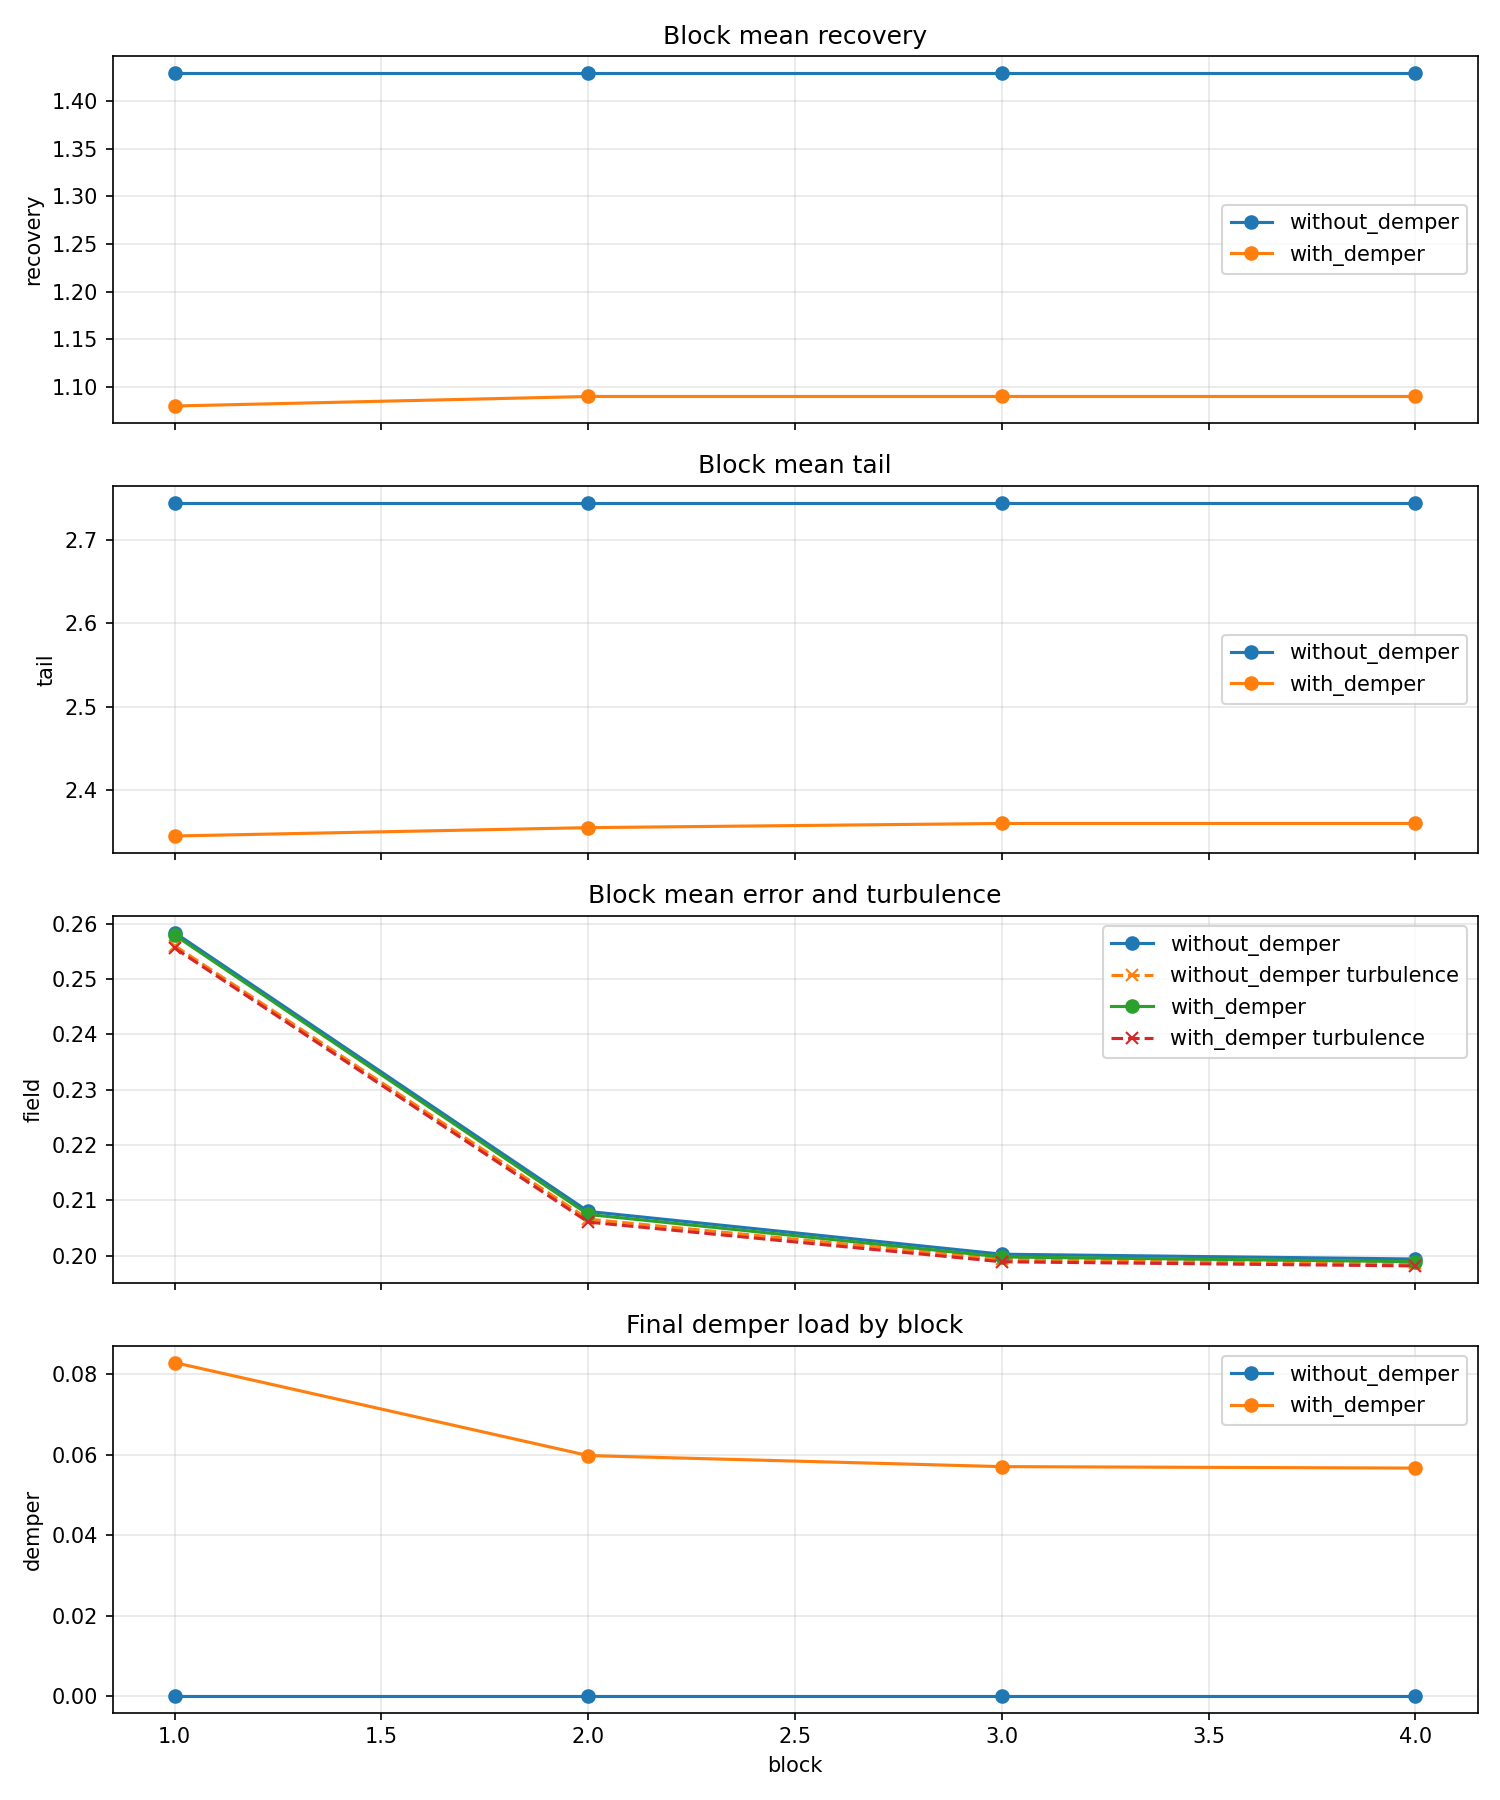
\includegraphics[width=0.95\linewidth]{figures/demper_ablation_plot.png}
    \caption{Buffered recovery (demper) ablation. This is the first mechanism in the current line to improve both recovery time and recovery tail while preserving field quality.}
    \label{fig:vol5_demper}
\end{figure}

\begin{figure}[h]
    \centering
    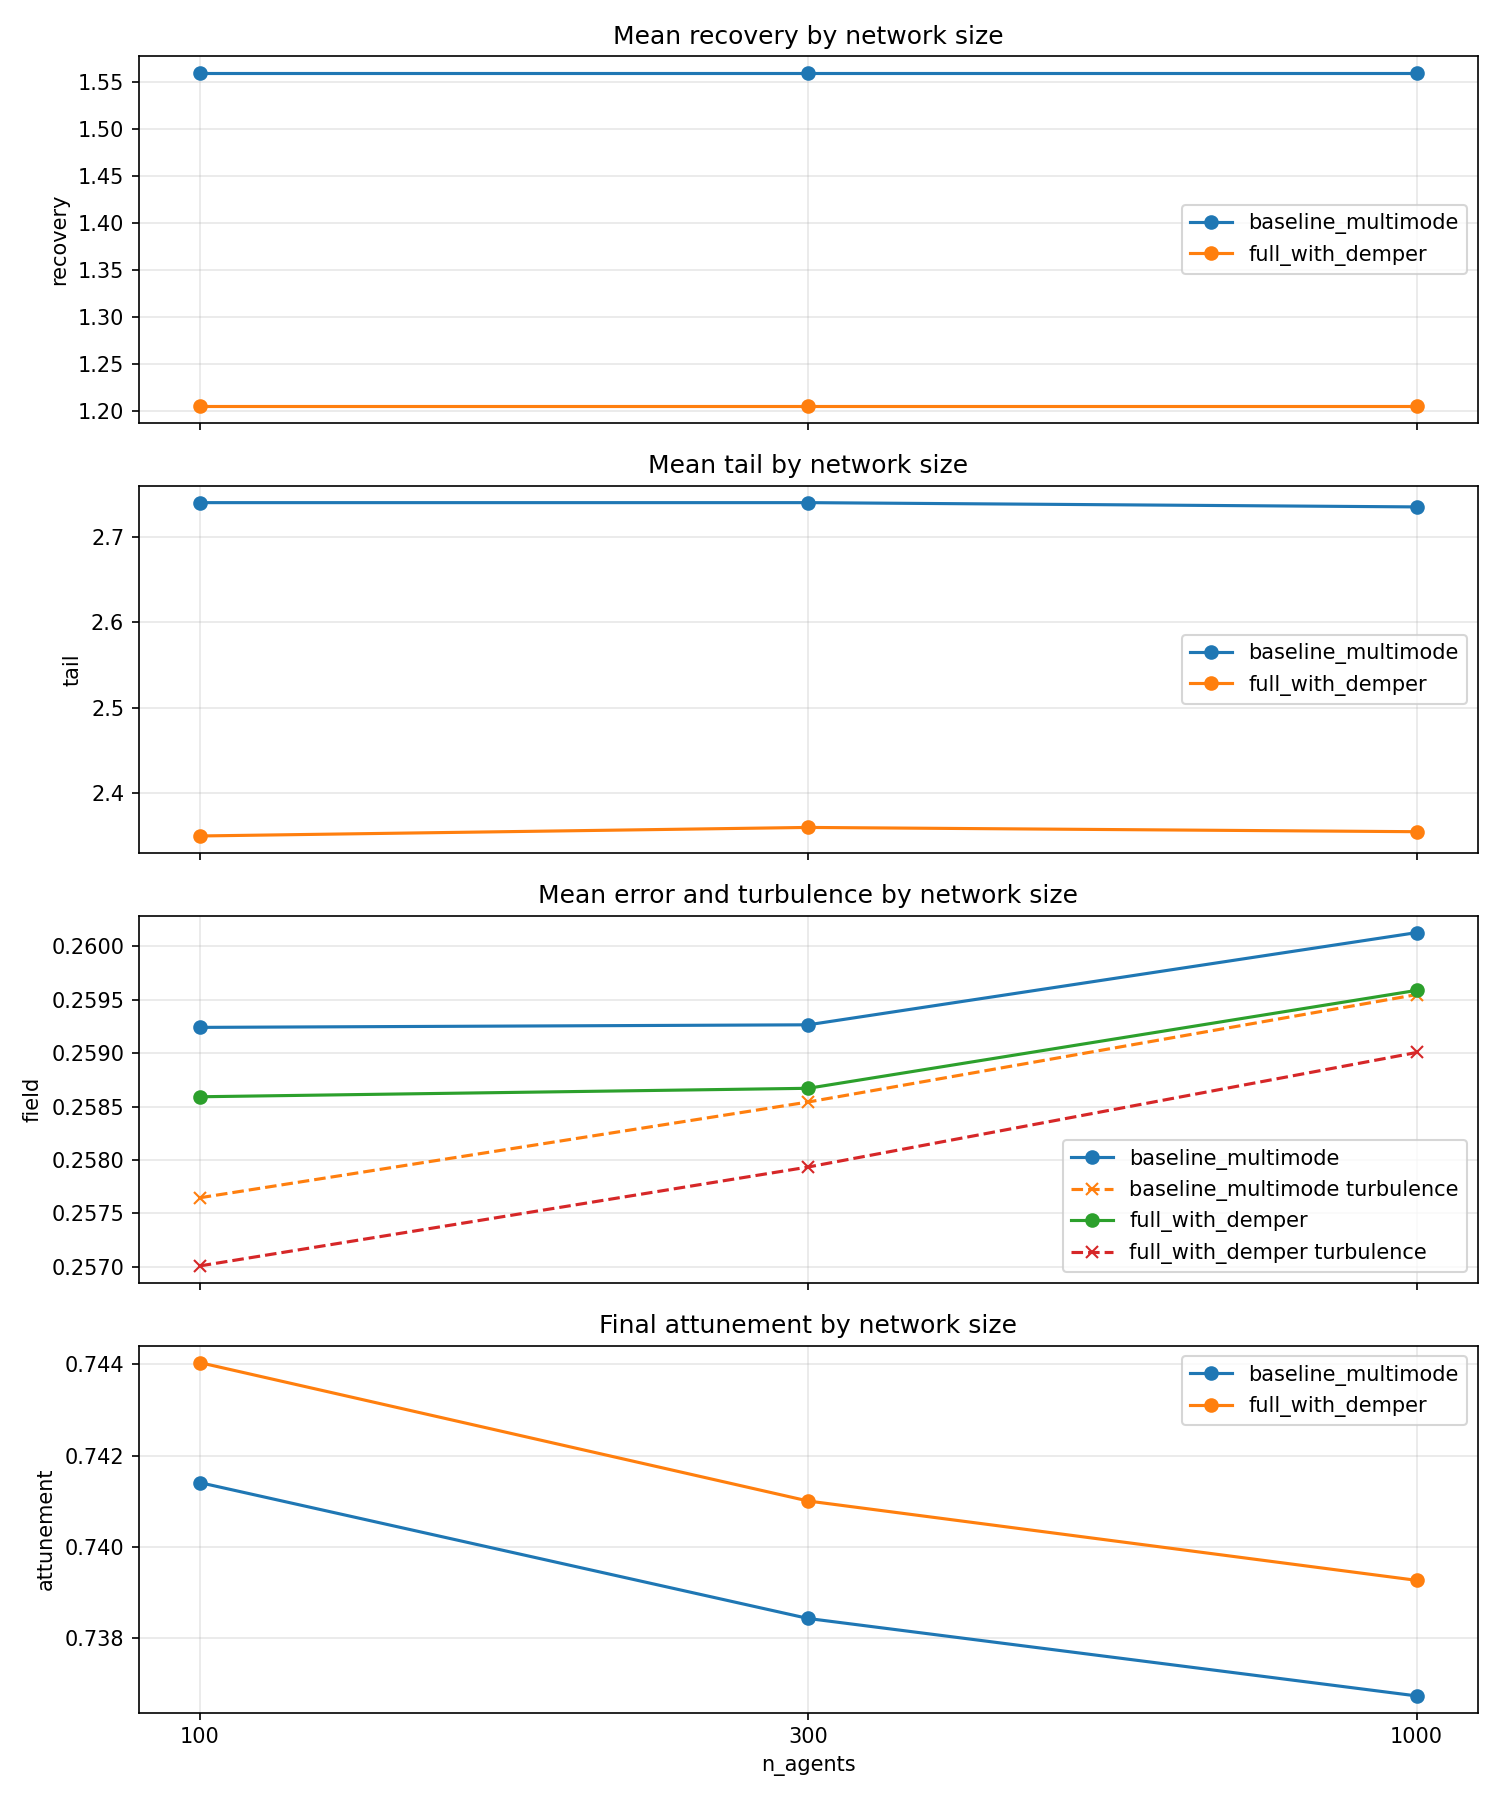
\includegraphics[width=0.95\linewidth]{figures/large_scale_validation_plot.png}
    \caption{Large-scale validation at $N=100$, $N=300$, and $N=1000$. The full model retains its recovery and tail advantage over the baseline multimode architecture.}
    \label{fig:vol5_large_scale}
\end{figure}

\section{Current Limits}
The present simulations still do not justify a mature theory of long-horizon group learning in the strongest sense, nor a completed memory architecture. Group memory remains weaker than the interaction-side mechanisms. Early focus-lock and simple rerouting attempts were not strong enough and are not treated as primary results. In addition, direct comparison against the old extreme RC boundary regime suggests that the new architecture softens the field there, but does not yet fully ``conquer'' the harshest published boundary zone by the old recovery criterion. The newer pause, attention, and recognition refinements make that limit more informative, not less: they suggest that the architecture can become earlier and more pattern-sensitive without yet becoming a full crisis-route learner. At the current stage, the most defensible center of Volume V is therefore a layered architecture: state-aware coordination, mutual attunement, multimode instruction, buffered recovery, and the first minimal signs of anticipatory instructor refinement.

\section{Conclusion}
The main contribution of Volume V is not a fully mature learning controller, but a bounded instructor-like coordination framework for heterogeneous networks that now has several aligned layers of support. Mutual attunement reduces field error. Multimode instruction improves heterogeneous heavy lessons more consistently than a monotone instructor signal. Long curriculum causes quality gains to accumulate over time. Buffered recovery (demper) finally shortens both recovery time and recovery tail. These gains remain visible at larger scales up to $N=1000$.

The practical claim of the present preprint should therefore remain disciplined but stronger than before: Volume V does not yet present a final theory of group learning, but it does present a coherent architecture in which heterogeneous groups become easier to coordinate through repeated interaction, differentiated guidance, and post-crisis release. In the current line, adaptive RC helps the field gather, attunement helps the group understand, multimode instruction helps the system respond to different failure types, buffered recovery helps the field let go after crisis, and the newest boundary refinements suggest how an instructor may begin to recognize and gather a labile field earlier. Quality improves first, timing gains appear once buffered recovery is modeled explicitly, and boundary recovery remains an open limit rather than a concealed failure. That is a sufficiently strong and coherent result for a serious exploratory preprint, and it gives the project a much more stable base for whatever comes next.

\end{document}
